\documentclass{anstrans}
%%%%%%%%%%%%%%%%%%%%%%%%%%%%%%%%%%%
\title{Parallel Performance of the Time Dependent Transport Code TDKENO with Applications to TREAT Simulations}
\author{Zander Mausolff,$^{*}$ Mark DeHart,$^{\dagger}$ Sedat Goluoglu $^{*}$}

\institute{
$^{*}$Nuclear Engineering Program, University of Florida
\\
529 Gale Lemerand Dr., Gainesville, FL, 32611
\and
$^{\dagger}$Nuclear Systems Design and Analysis Department Idaho National Laboratory 
\\
2525 North Freemont Street, Idaho Falls ID, 83415
}

\email{zanderm@ufl.edu $^{*}$} 


% Optional disclaimer: remove this command to hide
%\disclaimer{Notice: this manuscript is a work of fiction. Any resemblance to
%actual articles, living or dead, is purely coincidental.}

%%%% packages and definitions (optional)
\usepackage{graphicx} % allows inclusion of graphics
\usepackage{booktabs} % nice rules (thick lines) for tables
\usepackage{microtype} % improves typography for PDF

\newcommand{\SN}{S$_N$}
\renewcommand{\vec}[1]{\bm{#1}} %vector is bold italic
\newcommand{\vd}{\bm{\cdot}} % slightly bold vector dot
\newcommand{\grad}{\vec{\nabla}} % gradient
\newcommand{\ud}{\mathop{}\!\mathrm{d}} % upright derivative symbol

\begin{document}
%%%%%%%%%%%%%%%%%%%%%%%%%%%%%%%%%%%%%%%%%%%%%%%%%%%%%%%%%%%%%%%%%%%%%%%%%%%%%%%%
\section{Introduction}
Renewed interest in high fidelity simulation of excursion events has prompted the improvement of codes that solve the time-dependent Boltzmann transport equation. Often these codes make approximations to the transport equation in order to achieve results in a reasonable amount of time.  One such method, the improved quasi-static (IQS), makes few approximations compared to adiabatic, diffusion, point kinetics, etc \cite{Henry}. This is the approach taken by the code TDKENO \cite{Bentley}.  One downside to this approach is a portion of the calculation (flux shape) is done with a Monte Carlo code and must be called upon several times.  To minimize run time the flux shape calculation is solved with a modified version of KENO-VI from Scale 6.2  \cite{rearden2013overview}. This version of KENO runs in parallel across hundreds of nodes, thus improving performance.

The parallel capabilities of KENO allows TDKENO to simulate complex transient experiments with a large number of histories. These improvements are applied to the simulation of TREAT calibration experiments. 

%%%%%%%%%%%%%%%%%%%%%%%%%%%%%%%%%%%%%%%%%%%%%%%%%%%%%%%%%%%%%%%%%%%%%%%%%%%%%%%%
\section{Theory}
Solving the transport equation is non trivial when including the time dependence and the explicit representation of delayed neutrons. Transient simulations resulting in significant changes in the flux profile require rigorous methods to solve this "master equation" of reactor physics.  In TDKENO, the IQS method enables such simulations.  Utilizing the IQS method relies on the assumption that the total neutron flux can be factored into a shape and amplitude function \cite{goluoglu2001time}\cite{Gehin}.  
\begin{equation}
\label{factor}
    \phi(\bar{r},\bar{\Omega}',E,t) = A(t)\Psi(\bar{r},\bar{\Omega}',E,t)
\end{equation}

To make this definition unique to following definition is employed \cite{Henry}.  
\begin{equation}
    \label{unique}
    \iiint \frac{1}{v} \Psi(\bar{r},\bar{\Omega}',E,t)\phi^*(\bar{r},\bar{\Omega}',E,t) = constant
\end{equation}
This quantity should stay consistent in time to give the rest of the calculation merit.

The amplitude function captures the time dependence and takes on physical significance by being cast into the form of the point kinetics equations as follows:

\begin{equation}
    \label{eq:pt_kin}
    \frac{dA(t)}{dt} = \frac{\rho(t)-\bar{\beta}(t)}{\Lambda(t)} A(t) + \sum_{j=1}^{6} \lambda_jC_j(t) + \bar{Q}(t)
\end{equation}

where $A(t)$ is the amplitude function, $\rho$ is reactivity, $\bar{\beta}$ is the effective delayed neutron fraction, $\Lambda$ is the generation time, $\lambda_j$ is the decay constant per neutron group $j$, $C_j$ is the density of delayed neutron precursors for group j, and $\bar{Q}$ is a source.  
 Reactivity, generation time, etc. (referred to as reactivity calculations) in TDKENO are found from their inner product definitions using a linearly interpolated flux shape \cite{Bentley}.  Alternatively, these values may be computed during the Monte Carlo random walk but requires significant neutron histories to achieve low uncertainties \cite{Waddell}.  The shape function varies slowly in time and solves a modified version of the steady state transport equation.  The shape equation takes on the form of an inhomogeneous equation with the source consisting of a term representing the delayed-neutron precursor decay rate and a term from the backward difference approximation of the shape derivative.  In TDKENO the shape equation is solved via Monte Carlo, but in principle the shape equation may be solved with deterministic methods.  Reference \cite{Shayesteh} provides an excellent rationale for implementing Monte Carlo techniques in flux shape calculations.  For the complete derivation of the IQS method used in TDKENO, one can refer to the appendix in reference \cite{Bentley}. 

Applying the factorization in \ref{factor} to the three-dimensional time-dependent transport equation including delayed neutron results in a set of coupled equations.  Equations for the flux shape, amplitude, and delayed neutron precursors are solved on several time scales through an iterative process. The relative sizes are shown in Figure \ref{fig:time_scale}. 

\begin{figure}[h]
    \centering
    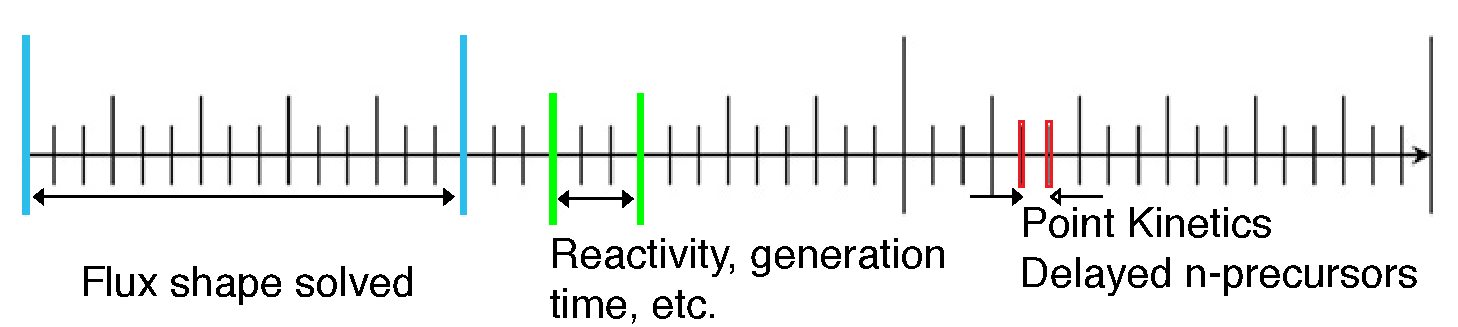
\includegraphics[width=8cm]{figures/time_scale.pdf}
    \caption{Time scale variation for IQS.}
    \label{fig:time_scale}
\end{figure}

The advantage of varying these time scales is computational overhead when compared to direct integration.  This comes from the flux shape being solved on a large time step. It is only done when the spatial distribution of neutrons changes significantly.  In between flux shapes, equation \ref{eq:pt_kin} is solved to capture the time dependent quantities such as power.   

%%%%%%%%%%%%%%%%%%%%%%%%%%%%%%%%%%%%%%%%%%%%%%%%%%%%%%%%%%%%%%%%%%%%%%%%%%%%%%%%
\section{Results and Analysis}
With the integration of the latest version of KENO from SCALE 6.2 we now have the ability to calculate the most intensive portion of the calculation in parallel (flux shape) \cite{rearden2013overview}.  Previously, for problems with complex geometry, the calculation of the shape may have taken several days or weeks to achieve adequate sampling and statistics.  By running TDKENO at the University of Florida's recently upgraded "HiperGator 2" supercomputer, we are able to run on hundreds of cores. As a result, these same calculations are only taking several hours. We apply these improvements to the challenging problem of simulating the experiments done at the Transient Reactor Test Facility (TREAT). 

To evaluate the performance of TDKENO, one of the M8CAL experiments is simulated.  The simulation is ran on a varying number of the HiperGator's nodes while keeping all other parameters specific to the problem constant.  Each node has an Intel E5-2698 v3 (16 core, 2.3 GHz) with 4GB of RAM per node. Note that at present, only the flux shape is calculated in parallel.  The amplitude function and related quantities are solved in serial. Investigation is underway to the potential of calculating these quantities on graphic processing units (GPUs).  

The M8CAL experiment modeled is referred to in the documentation as the temperature limited transient \#2855 \cite{Robinson_Bauer_1994}.  This experiment was chosen as it has proven to be the most difficult to simulate compared to similar transients as shown in \cite{physor_mausolff} and \cite{kontogeorgakos2014treat}.  Previous papers contained experimental data that was thought to have inconsistencies with the values reported in the M8CAL write up \cite{physor_mausolff}\cite{physor_paluch}.  However, upon further inspection, the data that corresponds to the M8CAL reported values has been found, digitized, and compared to the results shown here.

%%%%%%%%%%%%%%%%%%%%%%%%%%%%%%%%%%%%%%%%%%%%%%%%%%%%%%%%%%%%%%%%%%%%%%%%%%%%%%%%
\subsection{Computational Improvements}

The computational improvements are highlighted in TDKENO by running the same calculation on an increasing number of cores.  In this case, the KENO-VI calculations were run with 10000 particles per generation and 2500 generations. A total of 14 flux shapes were calculated with KENO at times primarily centered around the first few seconds.  We have chosen these parameters as they appear to give almost identical results to simulations run with many more histories.  This is shown in Figure \ref{fig:compare_hist}.  Simulations run with additional histories do result in less statistical uncertainties in values such as fluxes, $k_{eff}$, etc.  These are of less interest in this paper.  

\begin{figure}[h]
    \centering
    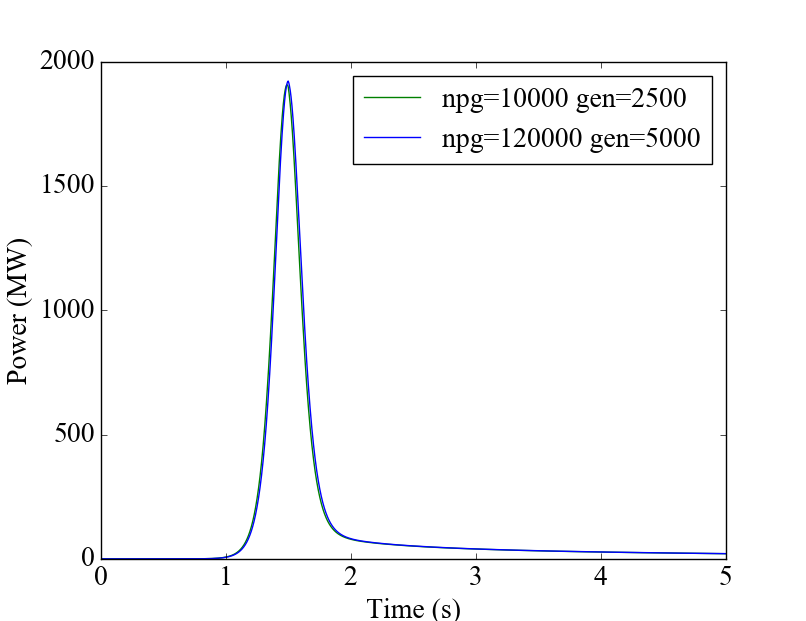
\includegraphics[width=9cm]{figures/comp_npg2855.png}
    \caption{The calculated power vs. time is compared between TDKENO simulation of TREAT transient \#2855 with differing numbers of histories. }
        \label{fig:compare_hist}
\end{figure}

The KENO-VI TREAT model used contains approximately 4000 regions with 21 materials.  The TREAT core is unique in its ability to safely simulate large reactivity insertions.  It accomplishes this with a core composed of 93.1\% $UO_2$ embedded in a graphite matrix, with a ratio of $UO_2$ to graphite of approximately 1:10000.  Details about the TREAT core may be found in \cite{bess2015baseline}.  A variety of control rods are available and the transient shown in this paper is induced by the rapid withdrawal of transient rods over 0.13 seconds. 

Below we show the affect of increasing the number of cores the problem is run on.  The relatively low number of histories results in poor scaling to large number of cores, as in Figure \ref{fig:speedup} due to increased communication time.  The communication time is compounded because the flux shape calculation is done in parallel and then gathered on a single core 14 times.  This master processor then computes the point kinetics values in serial.  Nevertheless the performance is drastically improved when compared to serial even with a modest amount of processors (for high performance computing standards).  
\begin{table}[h]
    \centering
    \begin{tabular}{c|c}
                    Total Cores  & Elapsed Time (minutes) \\
                    \hline 
                    1                  &   12,347            \\
                    16                 &   1,560             \\
                    32                 &   1,619              \\
                    48                 &   1,356              \\
                    64                 &   1,051             \\
                 %   80                 &                \\  
                    96                 &   917             \\
                    160                &   810             \\
                    \hline
    \end{tabular}
    \caption{Variation of the number of cores run for the simulation of \#2855. Elapsed time generated from the SLURM submission system \cite{yoo2003slurm}. }
    \label{tab:parallel}
\end{table}

Figure \ref{fig:speedup} plots the speed up compared to the number of cores run on.  Here, speedup is defined as the execution time on a single core divided by the time for that respective run.  Improvements could be made to further optimize the inputs by judiciously choosing the number of particles such that an integer amount are simulated on a single core.  Such methods may improve load balancing and communication time.  However, this is something a user should not be thinking about and these results are more indicative of "real world" behaviour. 

\begin{figure}[h]
    \centering
    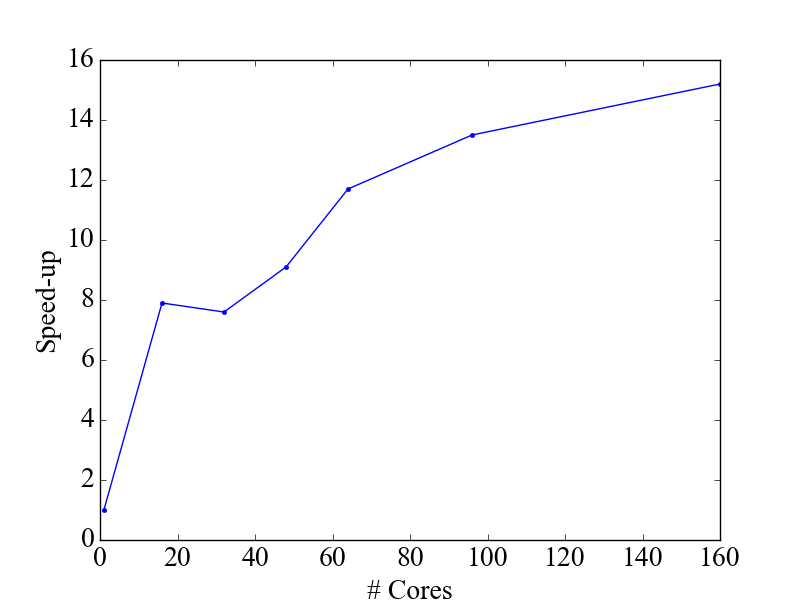
\includegraphics[width=9cm]{figures/speedup.png}
    \caption{Speed-up measured relative to the execution time on a single core.}
    \label{fig:speedup}
\end{figure}

%%%%%%%%%%%%%%%%%%%%%%%%%%%%%%%%%%%%%%%%%%%%%%%%%%%%%%%%%%%%%%%%%%%%%%%%%%%%%%%%

\subsection{Point Kinetics Variation}
As mentioned, the IQS methodology  splits the transport equation into several coupled equations solved on three time scales.  Each of the scales may be specified by the user.  The user defines when the flux shape updates are performed.  Next, an integer number of reactivity calculations and point kinetics solves are provided and are performed in-between flux shapes.  Note, the number of point kinetics solve specified refers to the number performed on between the reactivity calculations.  To illustrate, say 10 reactivity calculations and 20 point kinetics solved are given resulting in a total of 200 calculations in-between flux shapes.  The user may indicate the flux shape is updated at $1s$, $3s$, and $11s$.  In this case change in time between flux shapes would be $2s$ and $8s$ with 200 calculations in-between each.  So while the number of calculations between flux shapes is constant the time scale they are solved on may differ.  To visualize this we modify Figure \ref{fig:time_scale} below.

\begin{figure}[h]
    \centering
    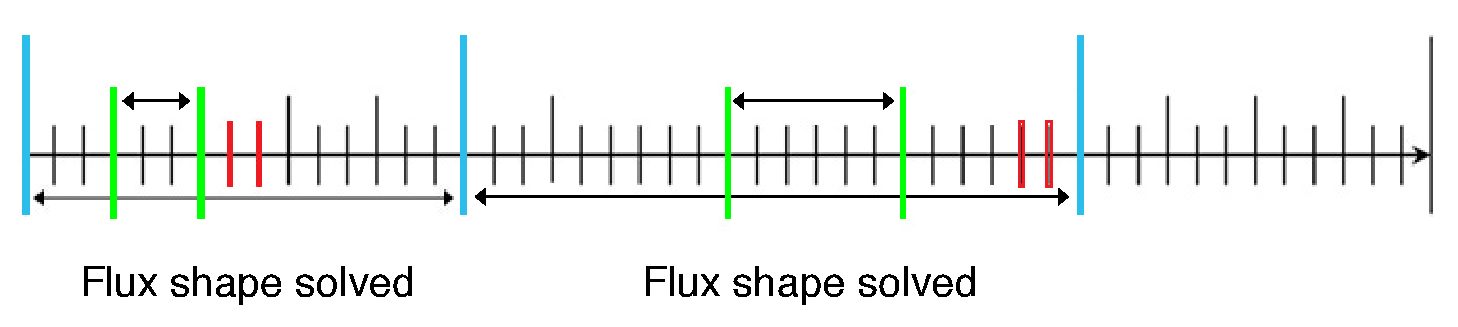
\includegraphics[width=8cm]{figures/time_scale_mod.pdf}
    \caption{IQS time scale modified to highlight varying flux shape update intervales.}
    \label{fig:time_scale_mod}
\end{figure}

As stated, the point kinetics equations are formulated to contain the time dependence to capture quantities such as power.  In its current state there are no methods to verify if too few calculations are chosen. To ensure time  behaviour is not omitted, we have been performing a large number of calculations between flux shapes.  Typically this is not as intensive as the flux shape calculation.  However, analyzing complex models results in geometries with thousands of regions. The number of regions is directly proportional to the calculation time as each regions reactivity, generation time, etc. must be integrated over the number of regions.  

One particular quantity of interest in the TREAT transient calibration experiments is the total energy deposited in the core.  Comparison of calculation to experiment is possible as the yield and power as a function of time are reported.  In previous  papers, the experimentally values were not transcribed properly and were slightly off \cite{physor_mausolff , physor_paluch}.  What is shown here aligns with the values provided in the original experimental report \cite{Robinson_Bauer_1994}. 
   
   To evaluate the sensitivity to the reactivity calculations, several simulations are performed.  These simulations vary the number of reactivity calculations between flux shapes while maintaining a constant number of point kinetics solves.  The first 10-90 reactivity calculations maintain the same number of solves(10) for the point kinetics equations.  The 100 line in Figure \ref{fig:ptkinvar} is what we have been using, with 100 point kinetics parameters calculations and 100 point kinetics solves. Choosing values beyond the typical one did not change the final answer.  To exemplify this a case with  500 point kinetics parameter updates and 500 point kinetics solves was run. Clearly this did not improve the solution as observed in Figure \ref{fig:ptkinvar}
   
   From about 10 to 50 reactivity calculations, there is an obvious deviation that gives a final yield far off from the experimental value.  After 60 point kinetics parameter calculations, further increases do not appear to give a different solution.  It appears one could get away with this many calculations and not suffer a loss of accuracy.

\begin{figure}[h]
    \centering
    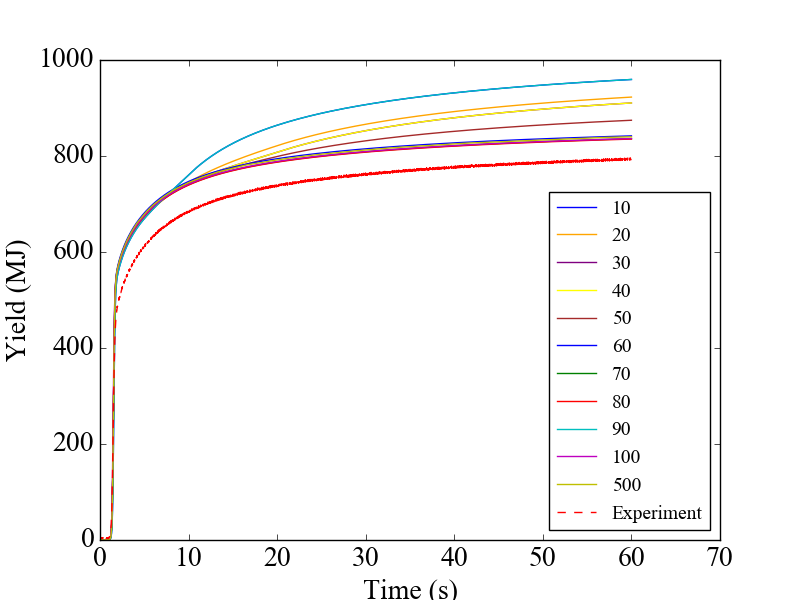
\includegraphics[width = 9 cm]{figures/ptkinvar.png}
    \caption{Varying the number of point kinetics parameter calculations between macro time steps.}
    \label{fig:ptkinvar}
\end{figure}

The goal behind minimizing the number of calculations in-between flux shape updates is computational savings.  To evaluate this we look at the total CPU time spent in-between flux shapes for the entire simulation.  This was done with a utility in TDKENO that measures the wall clock time between flux shapes and finds a total CPU time. We plot the calculation time for reactivity calculations 10-90 in Figure \ref{fig:ptkin_time}.  

\begin{figure}[h]
    \centering
    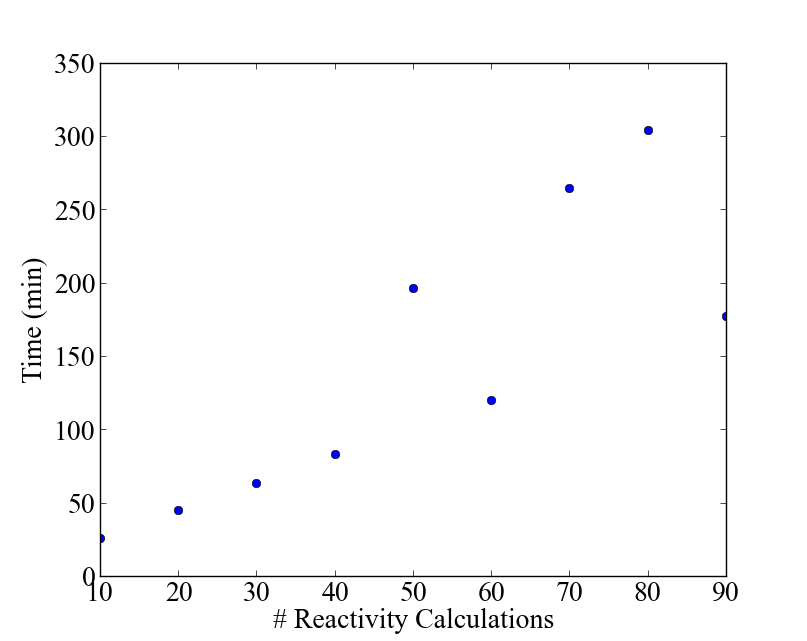
\includegraphics[width=9cm]{figures/ptkin_time_var.png}
    \caption{Total CPU time plotted against the number of point kinetics parameter calculations. }
    \label{fig:ptkin_time}
\end{figure}

There appears to be a linear trend in time as the number of reactivity calculations increases.  However, there are 3 outliers.  There is reason to believe these 3 runs are not representative of the general behaviour of TDKENO. The deviations may be attributed to running them on the HiperGator 2. These runs requested 5 nodes with 8 cores per node, which is only half the cores available on the node.  It is possible that during the runs, another program may have been using the other 8 cores and oversubscribed the node memory.  Other anomalies were observed in runs performed with the same parameters. The only difference being the number of cores run on.  For instance, looking at the CPU time for reactivity calculations on the runs shown in Figure \ref{fig:speedup} showed consistent behaviour, except for the run performed on a total of 80 cores as seen in Figure \ref{fig:ptkin_same_time}. These simulations were performed during the first month of operation of the HiperGator 2 and the system may not been optimized.  Figure \ref{fig:ptkin_same_time} shows the typical time (100 reactivity and 100 point kinetics calculations) spent  is approximately 300 minutes. Again in Figure \ref{fig:ptkin_same_time} has one calculation that took significantly longer.  Comparing the calculation time with typically chosen parameters to the minimum number required to get the same answer (60 reactivity calculations as per Figure \ref{fig:ptkin_time}) about 180 minutes could be saved.  

It is clear that minimizing the number of reactivity calculations improves computational time without sacrificing the final solution quality.  This motivates future work in several ways.  This time is not insignificant and can be further improved with parallelization on CPUs or GPUS.  Additionally, that determining solution convergence criteria is desirable to prevent unnecessary computational time.   

\begin{figure}[h]
    \centering
    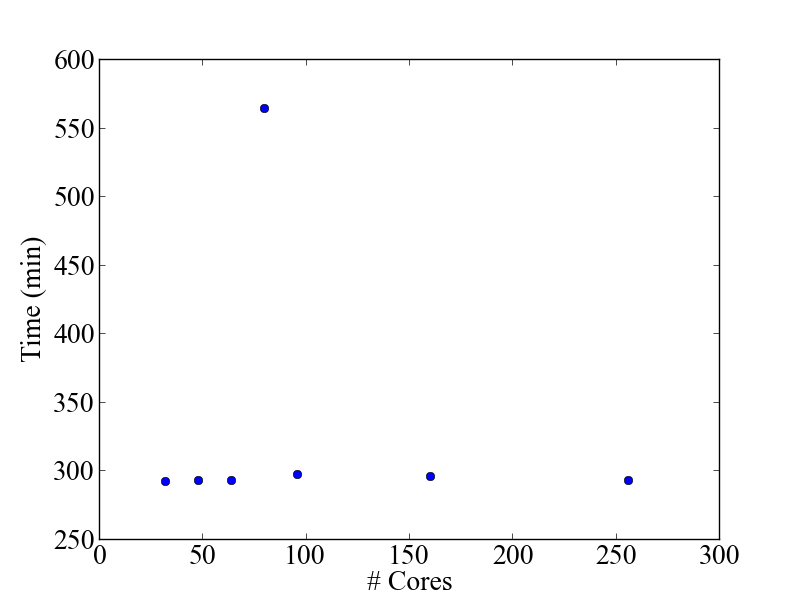
\includegraphics[width=9cm]{figures/comp_time_same-ptkin.png}
    \caption{Comparison of total CPU time for reactivity/point kinetics calculations while the number of cores each simulation is run on is varied.}
    \label{fig:ptkin_same_time}
\end{figure}

%%%%%%%%%%%%%%%%%%%%%%%%%%%%%%%%%%%%%%%%%%%%%%%%%%%%%%%%%%%%%%%%%%%%%%%%%%%%%%%%
\section{Conclusions}
The integration of a parallel flux shape solver has resulted in a transient analysis tool that is up to 15 times faster than previous implementations on a single core.  Nuanced behaviour such as the variation of reactivity calculations during a TDKENO run may now be studied in detail to further improve the method.  It has been shown for difficult problems like TREAT simulations, the deterministic portion of the code requires significant CPU time and are ripe for parallelization. Future work will be to determine convergence criteria for the reactivity and point kinetics calculations and have these done in parallel, likely on GPUs. 

%%%%%%%%%%%%%%%%%%%%%%%%%%%%%%%%%%%%%%%%%%%%%%%%%%%%%%%%%%%%%%%%%%%%%%%%%%%%%%%%

%%%%%%%%%%%%%%%%%%%%%%%%%%%%%%%%%%%%%%%%%%%%%%%%%%%%%%%%%%%%%%%%%%%%%%%%%%%%%%%%
\section{Acknowledgments}
This material is based upon work supported by the Idaho National Laboratory.

%%%%%%%%%%%%%%%%%%%%%%%%%%%%%%%%%%%%%%%%%%%%%%%%%%%%%%%%%%%%%%%%%%%%%%%%%%%%%%%%
\bibliographystyle{ans}
\bibliography{bibliography}

\end{document}

